\chapter{Data}
\label{chap:data}
In this chapter we introduce the data. Section \ref{section:data:data_description} offers a general description of the data used in this paper. The subsequent Section \ref{section:data:healthspan_target} outlines the selection process of diseases included in the target. In Section \ref{section:data:data_overview}, an overview of the collected information is provided. Next, in Section \ref{section:data:disease_incidence_ruling_censoring} we highlight our approach to defining disease incidence, and in Section \ref{section:data:feature_selection_and_preprocessing} we discuss the feature selection process. Lastly, in Section \ref{section:data:missing_data} we discuss how missing data is handled. 

\section{Lifelines}
\label{section:data:data_description}
The study was conducted with data from the Lifelines cohort, which is a large multi-generational study based in the northern part of the Netherlands \citep{Lifelines}. It was established by the UMCG in 2006, and primarily aims at gaining insight into the interactions between environmental, phenotypic and genotypic risk factors that affect the development of chronic diseases and healthy ageing. At baseline, data were collected for 167,729 participants ranging in age from 6 months to 93 years. The study involves regular physical examinations, cognitive tests, lung function and electrocardiogram (ECG), and extensive questionnaires completed every 5 years at a Lifelines location. In addition, participants complete follow-up questionnaires approximately every 1.5 years, providing insight into changes in behavior over time.
Exclusion criteria include severe psychiatric or physical illnes, a limited life expectancy ($<$ 5 years) or insufficient proficiency of the Dutch language. All participants signed an informed consent form before participation. Moreover, the Lifelines Cohort Study is conducted according to the principles of the Declaration of Helsinki and in accordance with research code of the UMCG.
%The data is provided by the University Medical Centre Groningen and the Lifelines research office and can be accessed via a secure Linux environment running on the high-performance cluster of the UMCG. 

\section{Healthspan}
\label{section:data:healthspan_target}
The target of the time-to-event analysis conducted in this paper is the incidence age of first disease from a shortlift of selected diseases. This incidence age is defined as the healthspan, or disease-free survival time of an individual. The diseases on the shortlist are Chronic Obstructive Pulmonary Disease (COPD), stroke, diabetes, heart failure and cancer. The diseases on the shortlist are selected based on a number of criteria. 

%1. They should be approximately (!!) equally severy, have the same impact on QoL. 
%2. Global Burden of Disease \cite{GBD}
Firstly, the diseases are selected based on their chronic nature, and their relative burden expressed in disability-adjusted life years (DALYs). In addition, they are highly associated with mortality and have a high risk factor attribution according to the Global Burden of Disease \citep{GBD}. The \cite{WorldHealthOrganization} defines one Disability-Adjusted Life Year (DALY) as representing the loss of the equivalent of one year of healthy life. The DALYs for a particular disease are the sum of the years of life lost due to premature mortality (YLLs) and the years lived with a disability (YLDs) due to prevalent cases of the disease in a population. DALYs are commonly used globally, and they offer a more complete picture of disease burden compared to mortality alone. All  diseases on the shortlist are among the top 8 'level-3' (the second last granularity level) diseases that account for the total DALYs, as can be seen in Table \ref{table:data:global_burden_of_disease}. This table contains the disease attributed percentage of total DALYs, and the risk factor attribution percentage. The Global Burden of Disease study is led by the Institute of Health Metrics and Evaluation at the University of Washington, and is the most comprehensive observational epidemiological study to date. It tracks mortality and morbidity in 204 countries and is an important tool for understanding the changing health challenges that exist in the world.
% sterker maken https://www.thelancet.com/lancet/visualisations/gbd-compare 
% Table: change caption, should be informative enough to understand table at once
\vspace{0.5cm}
\begin{table}[H]
    \centering
    \caption{Top 8 impactful diseases based on Disability-Adjusted Life Years - GBD 2019}
    \begin{tabular}{lll}
        \cline{1-3}
         & DALYs attribution \% & Risk factor attribution \%\\ \cline{1-3}
    Tracheal, bronchus, and lung cancer   & 5.6 & 83.5 \\
    Ischemic heart disease   & 5.5 & 94.4 \\
    Chronic obstructive pulmonary disease  & 4.7 & 72.9 \\
    Low back pain   & 4.5 & 40.5 \\
    Stroke   & 4.0 & 84.1 \\
    Falls   & 3.2 & 48.9 \\
    Colon and rectum cancer   & 3.0 & 60.4 \\
    Diabetes mellitus   & 2.9 & 100 \\
    \cline{1-3}
    \end{tabular}
    \label{table:data:global_burden_of_disease}
\end{table}

Note that we did not select \textit{Low back pain} and \textit{Falls}, because of their relatively low risk factor attribution. We also did not discriminate between different types of cancer in our target, because of the limited granularity of cancer type data in Lifelines. Lastly, as ischemic heart disease is a major risk factor of heart failure, we use \textit{Heart failure} in our target.

%3. Nr of occurences / incidence / association with age 
%4. Analyze prevalence before start of study 
Secondly, the diseases are selected on their association with age and their prevalence and incidence numbers. The prevalence and incidence numbers of the diseases in Lifelines can be found in Table \ref{table:data:disease_prevalence_incidence}. 
%Moreover, this table contains the Pearson correlation coefficient of the disease with  all selected diseases strongly correlate with age. (correlatie coefficienten toevoegen).  --> Pearson correlation is not well-suited for assessing the association between a continuous variable (age) and a binary variable (disease indicator). 
\vspace{0.5cm}
\begin{table} [H]
    \centering
    \caption{Lifelines disease prevalence and incidence percentages}
    \begin{tabular}{lll}
    \cline{1-3}
                       & Prevalence & Incidence \\ \cline{1-3}
    Stroke             & 0.7\%            & 0.5\%                   \\
    Diabetes           & 2.5\%            & 1.9\%             \\
    COPD               & 5.4\%            & 2.1\%              \\
    Cancer (all types) & 4.6\%            & 2.6\%              \\
    Heart failure           & 0.7\%             & 1.6\%    \\  
    \cline{1-3}       
    \end{tabular}
    \label{table:data:disease_prevalence_incidence}
\end{table} 

Lastly, in the selection process, several clinical experts from the UMCG have been consulted. They agreed to the specified shortlist of diseases and actknowledge the power of using the defined healthspan target to study ageing. 

\section{Data Overview}
\label{section:data:data_overview}
The Lifelines cohort consists of 3 main assessments, and 4 intermediate assessments. Information on disease presence and development is collected through questionnaires. Baseline assessment 1a contains information on presence of a disease before start of study. Follow-up assessments 1b, 1c, 2a, 3a and 3b contain information on disease development since the last time a Lifelines questionnaire was filled in. This structure allows for determination of between what ages a disease has developed, based on the assessments that an individual participated in. Besides disease presence and development information, Lifelines contains extensive information on demographics, lifestyle, psychosocial aspects and haematological and biochemical measures. The majority of the data is collected during the baseline assessment, referred to as assessment 1a. The subsequent main assessments, 2a and 3a, primarily contain follow-up information, which overlaps significantly with the baseline assessment 1a. An overview of data that is collected through questionnaires and clinical visits can be found in the \cite{LLdatacatalogue}. An overview of the information collected in the baseline questionnaire can be found in Table \ref{table:appendix:data_overview_baselines}, and an overview of the measurements collected during the clinical visits can be found in Table \ref{table:appendix:data_overview_clinical_measures} in Appendix \ref{chap:appendix}. % Weet niet of dit stuk hier helemaal past? 

%The intermediate assessments, 1b, 1c, 2b, and 3b, include a smaller subset of information. An overview of the number of variables and overlapping variables before feature selection is provided in Table \ref{table:data:variable_overlap_before_preprocessing}: 

%\vspace{0.5cm}
%\begin{table} [H]
%    \centering
%    \caption{Overview of variables and overlap with baseline of all assessments}
%    \begin{tabular}{lll}
%        \hline
%        \multicolumn{1}{l}{Assessment} & \multicolumn{1}{l}{Nr of columns} & %\multicolumn{1}{l}{Nr of overlapping columns with 1a} \\ \hline
%        1a (*)                         & 2062                              & 2062                                                                      \\
%        1b                             & 120                               & 109                                                                       \\
%        1c                             & 118                               & 107                                                                       \\
%        2a                             & 982                               & 743                                                                       \\
%        2b                             & 43                                & %39                                                                        \\
%        3a                             & 1063                              & %802                                                                       \\
%        3b                             & 86                                & %76                                                                        \\
%        2a + 3a (**)                       & 1374                              & %980                                 
%    \end{tabular}
%    \begin{tablenotes}
%        \small
%        \item \hspace{1cm} * baseline assessment
%        \item \hspace{1cm} ** merged with inner join
%      \end{tablenotes}
%    \label{table:data:variable_overlap_before_preprocessing}
%\end{table}

\section{Disease Incidence Ruling and Censoring}
\label{section:data:disease_incidence_ruling_censoring}
The section provides an overview of the custom disease incidence ruling, which is illustrated in Figure \ref{fig:data:disease_incidence_ruling}. 

\begin{figure}[H]
    \centering
    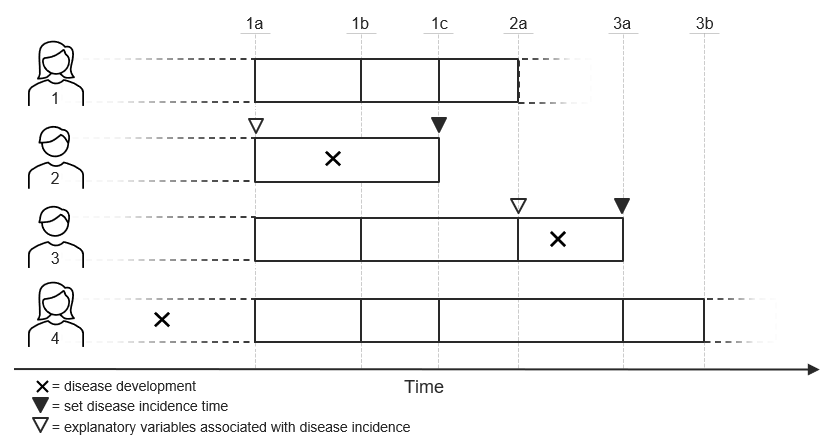
\includegraphics[width = 0.7\textwidth]{disease_incidence_ruling.png}
    \caption{Custom disease incidence ruling}
    \label{fig:data:disease_incidence_ruling}
  \end{figure}

In clinical studies where event status updates and covariates are collected during periodic follow-up assessments, censoring is very common. Generally, there are three variations; left-, right- and interval-censoring. Participants who have not developed a chronic disease before the end of the follow-up period are labeled as right-censored. In Figure \ref{fig:data:disease_incidence_ruling}, Participant 1 is right-censored. Right censoring can either occur due to end-of-study or due to loss-to-follow-up. When a participant enters the study with a disease of interest already present, this is a case of left-censoring. In Figure \ref{fig:data:disease_incidence_ruling}, this holds for Participant 4. Interval-censoring occurs when the event occurs in between two clinical assessments, and the exact time of incidence is unknown. It is assumed that censoring are non-informative about the event, regardless of the type of censoring. Left-censored individuals are not taken into account in the analysis, because it is impossible to evaluate the association of time-varying covariates with chronic disease incidence when the event has already occured. Moreover, the follow-up questions with which disease incidence is derermined are of the form: \textit{'Did the health problems listed below start since the last time you filled in a Lifelines questionnaire?'}. This question will inherently result in interval-censoring, because it does not provide the specific incidence time of disease. In addition, this question makes that disease incidence time is conditional on what assessments a participant took part in. 

The follow-up structure of the data and the target requires a custom disease incidence ruling and covariate matching approach. Not all participants have participated in every assessment, and for some participants disease development information or covartiates are missing for some assessments. Moreover, besides a set of constant covariates, there are measures that will vary over time and consequently over assessments. The effect of both the constant and time-varying variables on the outcome will be assessed in this paper. In order to do so, given the aforementioned missingness of data and censoring, custom rules of exlusion and disease incidence determination are required. The dataset scheme required for the time-varying Cox model is the \textit{long} format. This scheme contains one row per successive assessment set, including an ID, left (exclusive) timepoint, right (exclusive) timepoint, explanatory variables and an event indicator. The explanatory data is linked to the left timepoint, or the left clinical assessment of the set. The event indicator is linked to the right timepoint. This means that the explanatory data that is collected at a particular assessment, is linked to the time between that assessment and the next assessment, and is associated with the event occuring between those assessments or not. This logic is visualized in Figure \ref{fig:data:disease_incidence_ruling} for participants 2 and 3. This coding scheme assumes tht there is no interval-censoring. Furthermore, both age and time-on-study are included in the initial survival set, as well as an assessment and assessment difference indicator. This particular data structure allows for time-varying covariates. For example, the following example survival table in Table \ref{table:data:example_long_format} tracks thee individuals:
\vspace{0.5cm}
\begin{table} [H]
    \centering
    \caption{Example of a long format dataset with time-varying variables}
    \begin{tabular}{lllllllllll}
\hline
\textit{id} & \textit{start\_age} & \textit{stop\_age} & \textit{start} & \textit{stop} & \textit{var1} & \textit{var2} & \textit{ass\_start} & \textit{ass\_stop} & \textit{ass\_diff*} & \textit{event} \\ 
1  & 54         & 56        & 0     & 2    & 1    & 0.1  & 1a                & 1b               & 1                & 0     \\ 
1  & 56         & 57        & 2     & 3    & 1    & 0.2  & 1b                & 1c               & 1                & 0     \\ 
1  & 57         & 59        & 3     & 5    & 1    & 0.4  & 1c                & 2a               & 1                & 0     \\ 
2  & 26         & 27        & 0     & 1    & 0    & 0.4  & 1a                & 1b               & 1                & 0     \\ 
2  & 27         & 30        & 1     & 4    & 0    & 0.2  & 1a                & 1c               & 2                & 1     \\ 
3  & 69         & 70        & 0     & 1    & 0    & 0.3  & 1a                & 1b               & 1                & 0     \\ 
3  & 70         & 74        & 1     & 5    & 0    & 0.4  & 1b                & 1c               & 1                & 1     \\ \hline
    \end{tabular}
    \begin{tablenotes}
        \small
        \item* difference between start and stop assesment based on the sequence 1a, 1b, 1c, 2a, 3a, 3b
      \end{tablenotes}
    \label{table:data:example_long_format}
\end{table}

In this dataset, \textit{var1} is a time-independent variable and \textit{var2} is a time-dependent or time-varying variable. Given this format, individuals who have only participated in assessment 1a are excluded. Furthermore, participants that have a row where \textit{ass\_diff*} is larger than 2 are excluded. Including these participants would introduce too much uncertainty about the association between disease development and the time-varying covariates. Lastly, participants that have a missingness percentage over 75 are excluded, but this is discussed in section \ref{section:data:missing_data}. 

\section{Feature Selection and Preprocessing}
\label
{section:data:feature_selection_and_preprocessing}
%Beter onderbouwen methodes variable selection / preprocessing 
% convariates, factors, variables --> kiezen?? 
Given the high-dimensional nature of Lifelines, variable selection is a fundamental step in the modelling process. A parsimonous model will increase interpretation, and is therefore preferred. Nonetheless, we want to take into account as much information as possible, as Lifelines encompasses a wide range of potential predictors. To achieve this, features are selected based on existing literature and their relevance to research hypotheses. Additionally, dimensionality reduction techniques are employed to further reduce the feature space, as elaborated in the Methodology (section \ref{chap:methodology}). Moreover, in preprocessing, the time-variablity of the variables is analysed, and decisions are made on whether to allow a feature to be dynamic or not. 

In this study, features are selected based on a number of criteria. Predictors that are known to be associated with the risk of developing the diseases specified in the target are included in the analysis. The exclusion of such important factors will introduce omitted variable bias. Omitted variable bias entails that the model falsely attributes the effect of the omitted factors to the included variables. However, a certain amount of omitted variable bias is inevitable, as Lifelines is not an exhaustive study. Moreover, the presence of a feature in hypothesis automatically guarantees the inclusion of this feature in the analysis set. For example, it is hypothesized that the total amount of stress from long-term/chronic stressors experienced by the participant influences the development of disease. This factor is therefore included in the analysis set. 

In preprocessing, the time-variability of variables is assessed, and dynamic or static transformations are performed accordingly. The only variable that is static in Lifelines is gender. However, there are more variables that we take into account as static in analysis. Whenever a variable barely changes over time, it is set to a single value per individual by means of mean imputation. Moreover, when the dynamic nature of a variable is not of interest, a static tranformation is applied, and the variable is considered a constant throughout analysis. In the end, this method will result in a set of time-varying covariates, and a set of constant baseline covariates. It is essential that the time-varying variables are available in as many assessments as possible, as the applied method does not allow for empty values. Given that the explanatory data is linked to the left timepoint, and that assessment 2b does not contain disease development information, the maximum number of time-varying variables depends on the overlap of assessments 1a, 1b, 1c, 2a and 3a. However, when a certain variable is missing or empty in one of the follow-up assessments, the information will be imputated by carrying forward the most recent available information. This technique is called the last observation carried forward (LOCF) method. For example, when a participants' body mass index (BMI) is available in assessments 1a, 1c and 2a, the BMI of assessment 1b and 3a will equal the BMI measured in assessment 1a and 2a respectively. This method, as described in \cite{liu2006incorporating}, is selected because it safeguards the sample size and it is easily implementable. In order to fit the model that is applied in this study knowledge of all selected features at every potential event time is required. The LOCF technique prevents exclusion of participants for which a part of this information is missing, and therefore reduces selection bias. Selection bias, which is a side effect of visit-specific missingness, occurs when the population of participants with incomplete information is different from the population of participants with complete information. The downside of this method is that it also introduces bias by discretizing and pulling forward of continuously changing features. However, we conclude that the advantages associated with the LOCF method outweigh the limitations. Hence, this method is applied in order to maximize the sample size and allow more boundless inclusion of time-dependent effects.  

After feature selection and preprocessing, the remaining variable set will regularized further by the application of dimensionality reduction techniques. Hereafter they will be assessed on their significance and effect on the outcome. 

\section{Missing Data}
\label{section:data:missing_data}
Missing data is a prevalent phenomenon in clinical follow-up studies, and refers to the absence of information for certain features or observations for participants in the study. Missing data can arise due to various reasons such as participant attrition, loss to follow-up, or incomplete data collection. The occurrence of missing data poses challenges for researchers and can potentially introduce biases and affect the validity and reliability of study findings.

In clinical follow-up studies, missing data can be categorized into different types. Missing Completely at Random (MCAR) refers to missingness that occurs randomly and independently of any observed or unobserved data. It is the considered to be the strongest and most unrealistic type of missingness. Missing at Random (MAR) implies that the probability of missingness is dependent on observed data, but not on the unobserved data. Lastly, Missing Not at Random (MNAR) occurs when the probability of missingness is related to both observed and unobserved data, leading to potentially biased estimates. In this study, it is assumed that the missing data is MAR. Under this assumption, bias can be mitigated by applying appropriate imputation techniques. 

To address the issue of missing data in this study, various methods can be applied. These include complete case analysis, where only participants with complete data are included in the analysis. However, this results in a loss of information and a reduced sample size. Another approach is to perform imputation, which involves filling in missing values using statistical techniques. As introduced in section \ref{section:data:feature_selection_and_preprocessing}, missing constant data is imputed by means of mean imputation, and missing time-varying data is imputed by means of the LOCF technique. However, to minimize potential bias, participants who have more than 75\% imputed data are excluded. Due to the merging of the assessment datasets, and the fact that not all variables overalp assessments, the inherent missingness percentage of individuals is very high. Therefore, 75\% may seem extremely high, but this is relatively normal given the circumstances. More sophisticated imputation methods such as multiple imputation or maximum likelihood estimation are not considered in this study, as the aim of this study is to study factors associated to healthspan, and not to study data imputation techniques.  

Altoghether, it is important to note that while these methods help mitigate biases associated with MAR data, they rely on the assumption that the missingness mechanism is correctly specified. Moreover, mean imputation and LOCF are not the optimal imputation methods for MAR data, so biases may still persist. However, these methods do address the missing data in this study, and they aim to reduce bias by optimizing the sample size. This will in turn help to draw accurate conclusions regarding the association between features of interest and human healthspan. 